\input templates/header

\graphicspath{{figs/02/}}

\usepackage{cancel}
\usepackage{mleftright}

\def\arraystretch{1.1}

\newcommand*{\ballref}[1]{%
    \begin{pgfpicture}{-1ex}{-0.65ex}{1ex}{1ex}
    \usebeamercolor[fg]{item projected}
    {\pgftransformscale{1.75}\pgftext{\normalsize\pgfuseshading{bigsphere}}}
    {\pgftransformshift{\pgfpoint{0pt}{0.5pt}}
      \pgftext{\usebeamerfont*{item projected}\ref{#1}}}
  \end{pgfpicture}}%

\begin{document}

\title[ASD - Analisi di algoritmi]{\textbf{Algoritmi e Strutture Dati}\\[18pt]Analisi di algoritmi\\Funzioni di costo, notazione asintotica}


%-------------------------------------------------------------------------
\FrameTitle{}


\section{Notazione asintotica}

\subsection{Definizioni}

\begin{frame}{Notazioni $O$, $\Omega$, $\Theta$}

\vspace{-9pt}
\begin{myboxtitle}[Definizione -- Notazione $O$]
Sia $g(n)$ una funzione di costo; indichiamo con $O(g(n))$ l'insieme
delle funzioni $f(n)$ tali per cui:\\[-6pt]
\[
  \exists c>0, \exists m \geq 0: \alert{f(n) \leq cg(n)}, \forall n \geq m
\]
\end{myboxtitle}

\medskip
\begin{itemize}
\item Come si legge: $f(n)$ è “\alert{O grande}” (big-O) di $g(n)$
\item Come si scrive: $f(n) = O(g(n))$
\item $g(n)$ è un \alert{limite asintotico superiore} per $f(n)$
\item $f(n)$ cresce al più come $g(n)$
\end{itemize}

\end{frame}

\begin{frame}{Notazioni $O$, $\Omega$, $\Theta$}

\vspace{-9pt}
\begin{myboxtitle}[Definizione -- Notazione $\Omega$]
Sia $g(n)$ una funzione di costo; indichiamo con $\Omega(g(n))$ l'insieme
delle funzioni $f(n)$ tali per cui:\\[-6pt]
\[
  \exists c>0, \exists m \geq 0: \alert{f(n) \geq cg(n)}, \forall n \geq m
\]
\end{myboxtitle}

\medskip
\begin{itemize}
\item Come si legge: $f(n)$ è “\alert{Omega grande}”  di $g(n)$
\item Come si scrive: $f(n) = \Omega(g(n))$
\item $g(n)$ è un \alert{limite asintotico inferiore} per $f(n)$
\item $f(n)$ cresce almeno quanto $g(n)$
\end{itemize}
\end{frame}

\begin{frame}{Notazioni $O$, $\Omega$, $\Theta$}

\vspace{-9pt}
\begin{myboxtitle}[Definizione -- Notazione $\Theta$]
Sia $g(n)$ una funzione di costo; indichiamo con $\Theta(g(n))$ l'insieme
delle funzioni $f(n)$ tali per cui:\\[-6pt]
\[
  \exists c_1>0, \exists c_2>0, \exists m \geq 0: \alert{c_1g(n) \leq f(n) \leq c_2g(n)}, \forall n \geq m
\]
\end{myboxtitle}

\medskip
\begin{itemize}
\item Come si legge: $f(n)$ è “\alert{Theta}” di $g(n)$
\item Come si scrive: $f(n) = \Theta(g(n))$
\item $f(n)$ cresce esattamente come $g(n)$
\item $f(n) = \Theta(g(n))$ se e solo se $f(n) = O(g(n))$ e $f(n) = \Omega(g(n))$
\end{itemize}

\end{frame}

\begin{frame}{Graficamente}
  
\begin{center}
\vspace{-12pt}
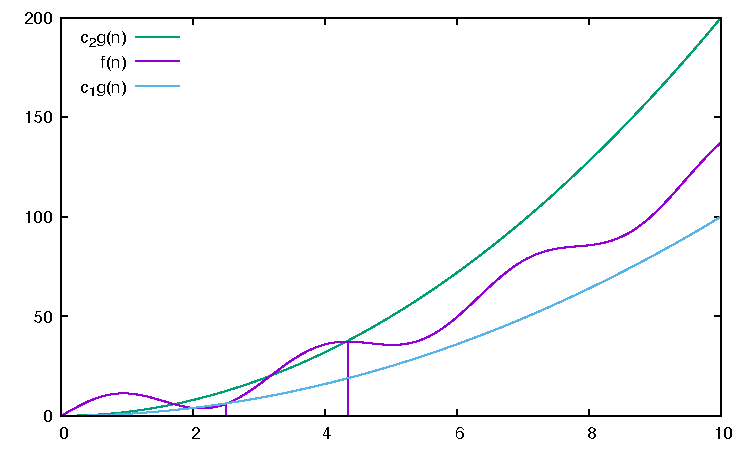
\includegraphics[width=0.9\textwidth]{plot-3.pdf}
\end{center}
  
\end{frame}


%\input analisi/funzioni-1.tex
\input analisi/funzioni-2.tex
\input analisi/funzioni-3.tex
\input analisi/funzioni-4.tex
\input analisi/funzioni-5.tex

\title[ASD - Analisi di funzioni]{\textbf{Algoritmi e strutture dati}\\[12pt]Analisi di funzioni\\Back to algorithms!}

%-------------------------------------------------------------------------
\FrameTitle{}

\section{Back to algorithms!}

%-------------------------------------------------------------------------
\begin{frame}[fragile]{Complessità della Versione 1}

\begin{columns}[T]
\column{0.52\textwidth}
\small
\begin{lstlisting}[language=java]
int maxsum1(int[] A, int n) {
  int maxSoFar = 0;
  for (int i=0; i < n; i++) {
    for (int j=i; j < n; j++) {
      int sum = 0;
      for (int k=i; k <= j; k++) {
        sum = sum + A[k];
    }
    maxSoFar = max(maxSoFar, sum);
    }
  }
  return maxSoFar;
}
\end{lstlisting}
\column{0.46\textwidth}
La complessità dell'algoritmo può essere approssimata come segue (contando
il numero di esecuzioni della riga più interna)
\[
T(n) = \sum_{i=0}^{n-1} \sum_{j=i}^{n-1} (j-i+1)
\]
\end{columns}

\end{frame}

%-------------------------------------------------------------------------
\begin{frame}{Complessità della Versione 1 - $O(n^3)$}

Vogliamo provare che  $T(n) = O(n^3)$, i.e.

\[
  \exists c_2 > 0, \exists m \geq 0: T(n) \leq c_2 n^3, \forall n \geq m
\]

\vspace{-12pt}
\begin{align*}
T(n) &= \sum_{i=0}^{n-1} \sum_{j=i}^{n-1} (j-i+1) \\
     &\leq \sum_{i=0}^{n-1} \sum_{j=i}^{n-1} n 
     \leq \sum_{i=0}^{n-1} \sum_{j=0}^{n-1} n \\
     &= \sum_{i=0}^{n-1} n^2 
     = n^3 \leq c_2n^3
\end{align*}

Questa disequazione è vera per $n \geq m = 0$ and $c_2 \geq 1$.

\end{frame}

%-------------------------------------------------------------------------
\begin{frame}{Complessità della Versione 1 - $\Omega(n^3)$}

\small
Vogliamo provare che  $T(n) = \Omega(n^3)$, i.e.

\[
  \exists c_1 > 0, \exists m \geq 0:  T(n) \geq c_1 n^3, \forall n \geq m
\]

\vspace{-12pt}
\begin{align*}
T(n) &= \sum_{i=0}^{n-1} \sum_{j=i}^{n-1} (j-i+1) \\
     &\geq \sum_{i=0}^{n/2} \sum_{j=i}^{i+n/2-1} (j-i+1) \\ 
     &= \sum_{i=0}^{n/2} \sum_{j=i}^{i+n/2-1} n/2 \\ 
     &= \sum_{i=0}^{n/2} n^2/4 \geq n^3/8 \geq c_1 n^3 
\end{align*}

L'ultima disequazione è vera per $n \geq m = 0$ and $c_1 \leq 8$.

\end{frame}

%-------------------------------------------------------------------------
\begin{frame}[fragile]{Complessità della versione 2}

\vspace{-18pt}
\begingroup
\small
\begin{lstlisting}[language=java]
int maxsum2(int[] A, int n) {
  int maxSoFar = 0;
  for (int i=0; i < n; i++) {
    int sum = 0;
    for (int j=i; j < n; j++) {
      sum = sum + A[j];
      maxSoFar = max(maxSoFar, sum);
    }
  }
  return maxSoFar;
}
\end{lstlisting}  
\endgroup

La complessità di questo algoritmo può essere approssimata come segue (stiamo contando il numero di passi nel ciclo più interno)
\[
T(n) = \sum_{i=0}^{n-1} n-i
\]


\end{frame}

\begin{frame}{Complessità della versione 2 - $\theta(n^2)$}

Vogliamo provare che $T(n) = \theta(n^2)$.

\begin{align*}
T(n) &= \sum_{i=0}^{n-1} n-i \\
     &= \sum_{i=1}^{n} i \\
     &= \frac{n(n+1)}{2} = \Theta(n^2)
\end{align*}

Questo non richiede ulteriori dimostrazioni

\end{frame}

%-------------------------------------------------------------------------
\begin{frame}[fragile]{Complessità della versione 3}

\footnotesize
\vspace{-6pt}
\begin{columns}[T]
\column{0.54\textwidth}
\vspace{-12pt}
\begin{lstlisting}[language=java]
int maxsum_rec(int[] A, int i, int j) {
  if (i==j) 
    return max(0, A[i]);
  int m = (i+j) / 2;
  int maxs = maxsum_rec(A, i, m);
  int maxd = maxsum_rec(A, m+1, j);
  int maxss = 0;
  int sum = 0;
  for (int k=m; k>=i; k--) {
    sum = sum+A[k];
    maxss = max(maxss, sum);
  }
  int maxdd = 0;
  sum = 0;
  for (int k=m+1; k<=j; k++) {
    sum = sum+A[k];
    maxdd = max(maxdd, sum);
  }
  return max(max(maxs,maxd),maxss+maxdd);
}


int maxsum3(int[] A, int n) {
  return maxsum_rec(A,0,n-1);
}
\end{lstlisting}  
\column{0.44\textwidth}
Per questo, definiamo la equazione di ricorrenza: \pause
\[
  T(n) = 2T(n/2) + n
\]
Utilizzando il teorema, possiamo vedere che $\alpha = \log_2 2 = 1$ e $\beta=1$, quindi $T(n) = \Theta(n \log n)$.
\end{columns}

\end{frame}


%-------------------------------------------------------------------------
\begin{frame}[fragile]{Complessità della versione 4}

\vspace{-18pt}
\begin{lstlisting}[language=java]
int maxsum4(int A[], int n) {
  int maxSoFar = 0;
  int maxHere = 0;
  for (int i=0; i < n; i++) {
    maxHere = max(maxHere+A[i],0);
    maxSoFar = max(maxSoFar,maxHere);
  }  
  return maxSoFar;
}
\end{lstlisting}  

E' facile vedere che la complessità di questa versione è $\theta(n)$.

\end{frame}

\subsection{Ruolo dei fattori molitplicativi}

%-------------------------------------------------------------------------
\begin{frame}{Fattori moltiplicativi}

\vspace{-9pt}	
\BB{
A volte, i fattori moltiplicativi di una funzione di complessità sono talmente alti che se ne sconsiglia l'uso per piccoli valori di $n$
}

\IG{0.65}{confronto.png}

\end{frame}

%-------------------------------------------------------------------------
\begin{frame}{GNU Multiple Precision Arithmetic Library}

\BI
\item Utilizzata da Mathematica, Maple, etc.
\item Le moltiplicazioni vengono realizzate utilizzando algoritmi diversi,
mano a mano che $n$ cresce.
\item \url{https://gmplib.org/manual/Multiplication-Algorithms.html}
\EI

\medskip
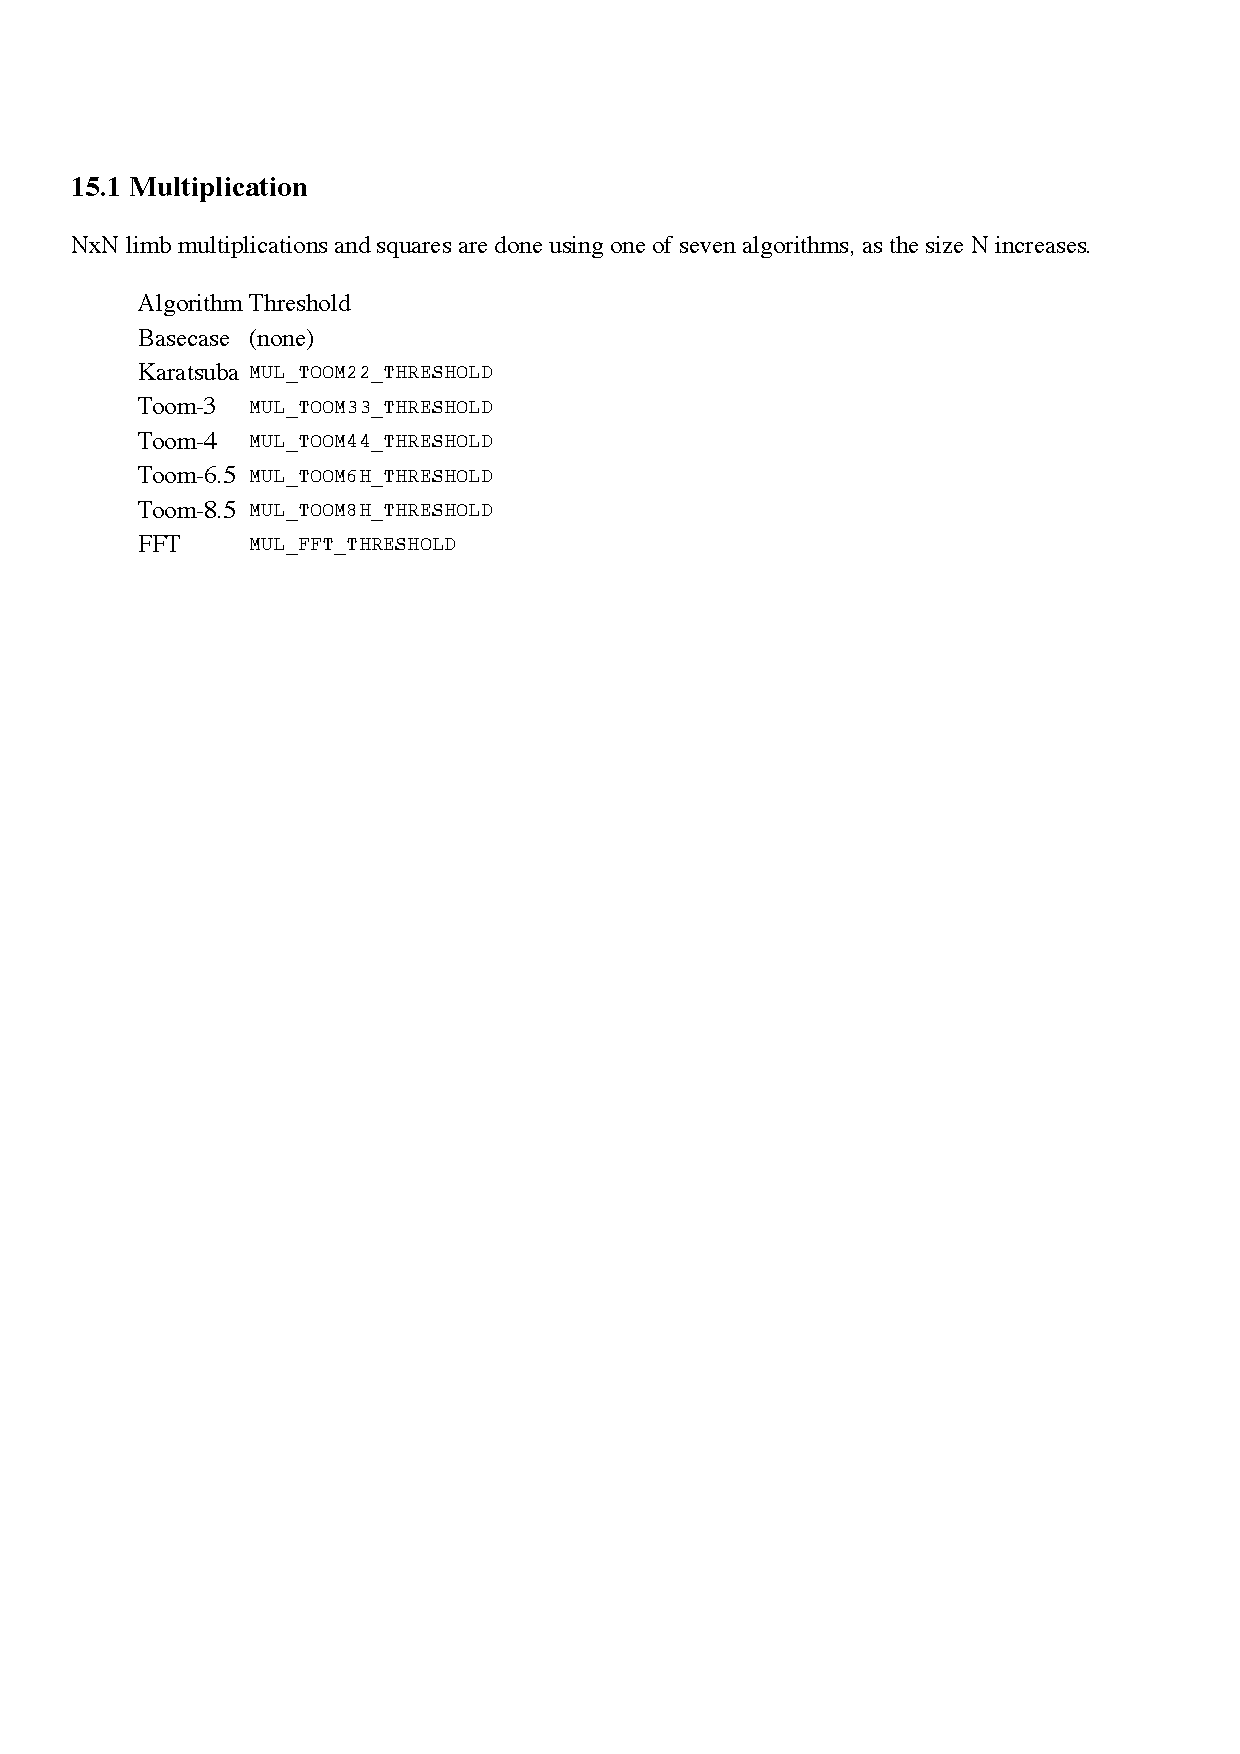
\includegraphics[width=\textwidth]{gmp.pdf}

\end{frame}


%-------------------------------------------------------------------------
\begin{frame}{GNU Multiple Precision Arithmetic Library}

\BI
\item Utilizzata da Mathematica, Maple, etc.
\item I limiti (threshold) dipendono dall'architettura
\EI

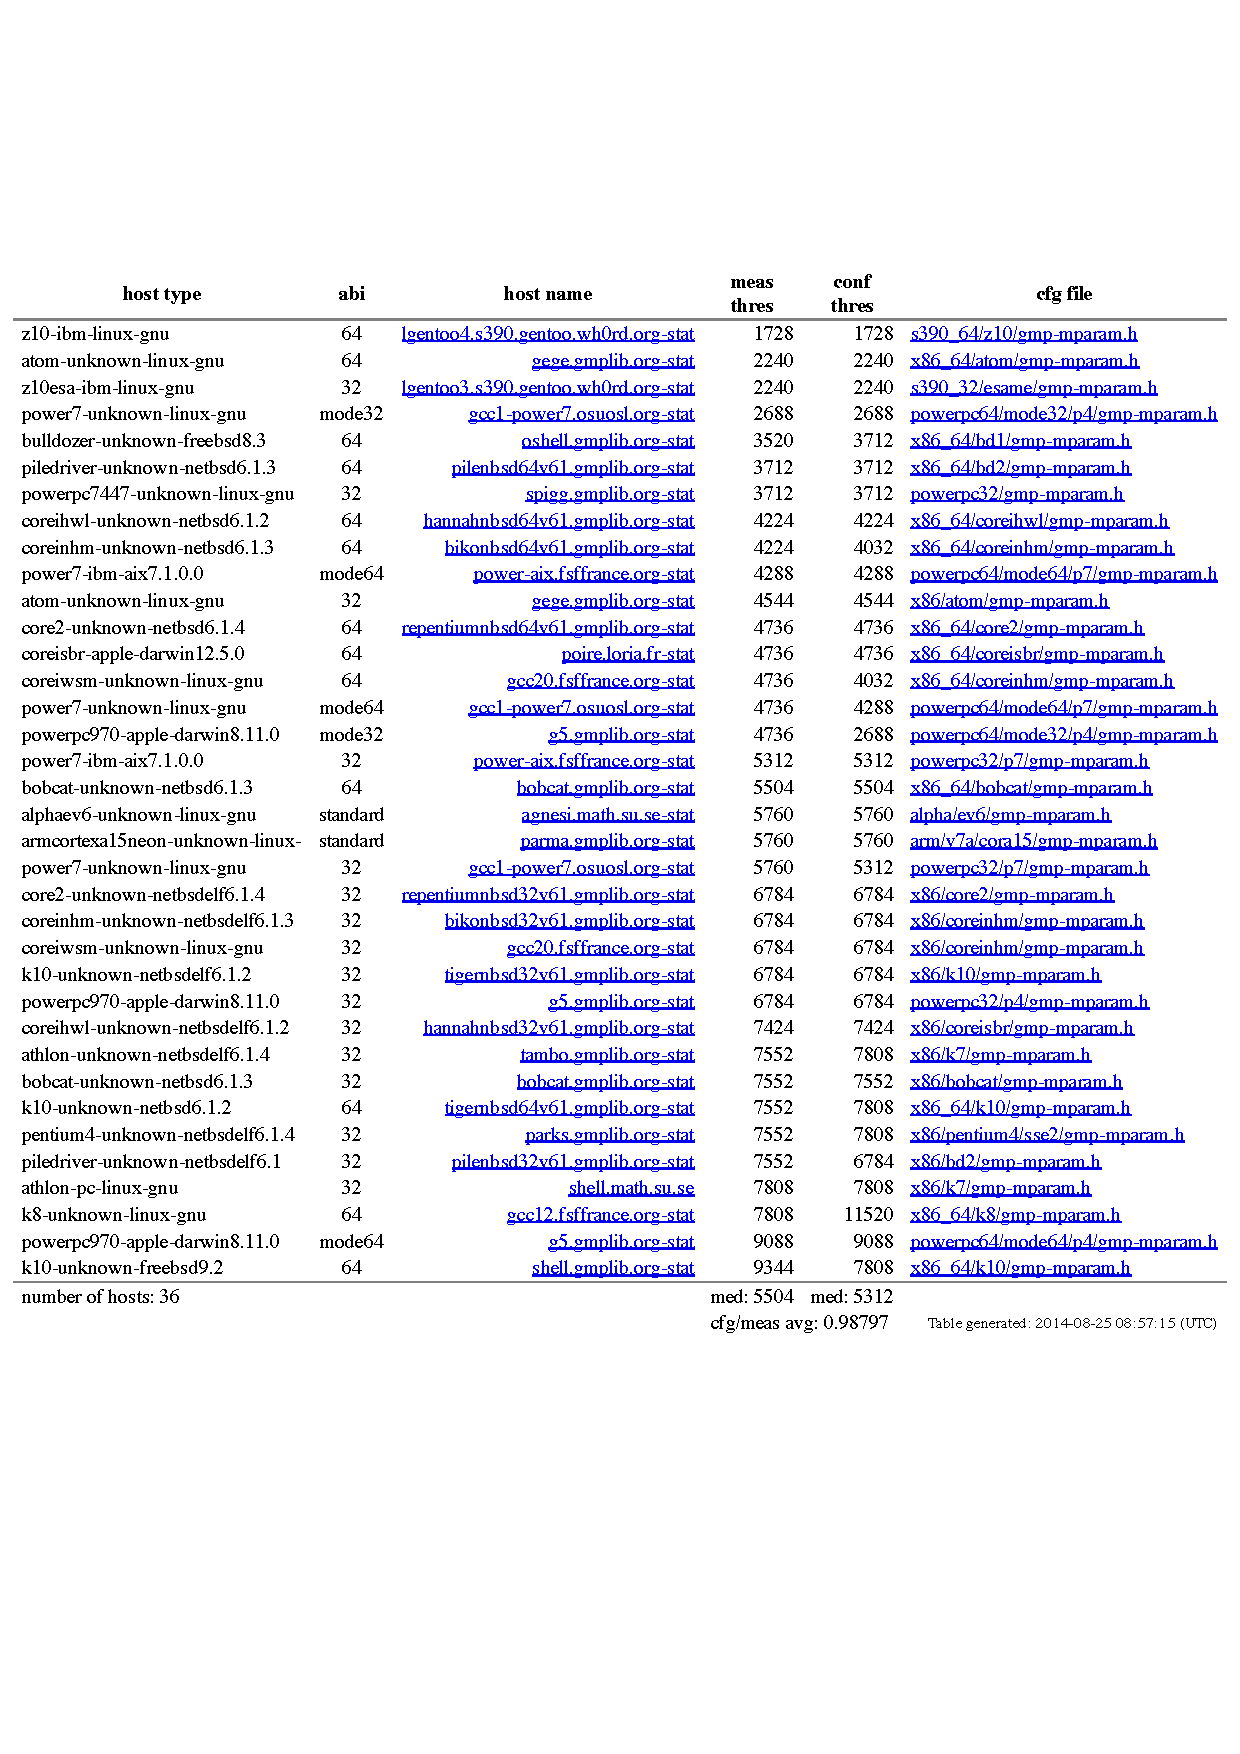
\includegraphics[width=\textwidth]{threshold.pdf}

\end{frame}


\end{document}